Bei der Beschreibung von Würfen, also von Flugbahnen von Körpern, wendet man die Bewegungsgesetze an und kombiniert diese falls notwendig.


\subsection{Vertikaler Wurf}

Der vertikale Wurf ist eine eindimensionale Bewegung, bei der ein Körper mit einer bestimmten Geschwindigkeit $v_0$ senkrecht nach oben geworfen wird und durch die Erdbeschleunigung wieder nach unten beschleunigt wird.

Daher lässt sich die Höhe des Körpers in Abhängigkeit der Zeit mit der \gleichungsreferenz{eq:streckegleichmaessig} beschreiben:

\begin{align} \label{eq:wurfvertikal}
	h(t) = -\frac{1}{2}g \cdot t^2 + v_0 \cdot t + h_0
\end{align}

\noindent Diese Gleichung kann gleich $0$ gesetzt werden um den Zeitpunkt zu erhalten, bei dem der Körper wieder auf der Erde aufschlägt. Um die Geschwindigkeit, mit der der Körper auftrifft zu erhalten, muss der errechnete Zeitpunkt in die Gleichung für die Geschwindigkeit (Siehe: \gleichungsreferenz{eq:geschwindigkeitgleichmaessig}) für $t$ und die negative Erdbeschleunigung ($-g$) für $a$ eingesetzt werden.


\subsection{Waagerechter Wurf}

Der waagerechte Wurf tritt bspw. ein, wenn ein Flugzeug Ladung abwirft.

Die Bewegung des Ladungskörpers in x-Richtung, also entlang der Flugrichtung, verläuft gleichförmig (Luftreibung wird ignoriert), also mit konstanter Geschwindigkeit $v_x$. Die Bewegung in y-Richtung ist, wie beim vertikalen Wurf eine gleichmäßig beschleunigte Bewegung mit der Erdbeschleunigung.

Folgende zwei Gleichungen sind zur Beschreibung nötig, wobei nicht mehr nur $h$, sondern $x$ und $y$ für die Strecken verwendet werden, da es ja nun 2 Richtungen gibt:

\begin{align}
	x(t) = v_x \cdot t
\end{align}

\begin{align}
	y(t) = -\frac{1}{2}g \cdot t^2 + y_0
\end{align}

\noindent Bei $x(t)$ wurde absichtlich die mögliche Anfangsstrecke weggelassen, zur Vereinfachung der weiteren Rechnung.

Nun ist es praktisch, nur eine Gleichung für die Beschreibung einer Bewegung zu haben. Dafür wird $x(t)$ nach $t$ umgestellt und dieses $t$ dann in $y(t)$  eingesetzt, sodass man eine Gleichung für die Höhe in Abhängigkeit von der Strecke in x-Richtung hat, was oft deutlich handlicher ist, als eine Gleichung für $y$ in Abhängigkeit der Zeit:

\begin{align}
\begin{split}
	x(t) &= v_x \cdot t \\
	t(x) &= \frac{x}{v_x}
\end{split}
\end{align}

\noindent Eingesetzt in $h(t)$:

\begin{align} \label{eq:waagerechtgesamt}
\begin{split}
	y(t) &= -\frac{1}{2}g \cdot t^2 + y_0 \\
	y(x) &= -\frac{1}{2}g \cdot \frac{x^2}{v_x^2} + y_0
\end{split}
\end{align}


\subsection{Schiefer Wurf}

Beim schiefen Wurf wird ein Körper unter einem Winkel geworfen, sodass dieser eine Wurfparabel beschreibt.

\begin{figure}[H]
	\centering
	\begin{comment} Gnuplot:
set xlabel "x"
set ylabel "y"
set output "schraeger_wurf.png"
set arrow 3 front to 2.5,3.125 size screen 0.025,22,60 filled ls 1
set arrow 4 front to 2.5,0 size screen 0.025,22,60 filled ls 1
set arrow 5 front to 0,3.125 size screen 0.025,22,60 filled ls 1
set label 1 "v_x" at 1.2,0.3 font 'Verdana,48'
set label 2 "v_0" at 1.2,2.25 font 'Verdana,48'
set label 3 "v_{y0}" at 0.1,1.7 font 'Verdana,48'
plot (-0.26*(x*x)+1.25*x) ls 1
	\end{comment}
	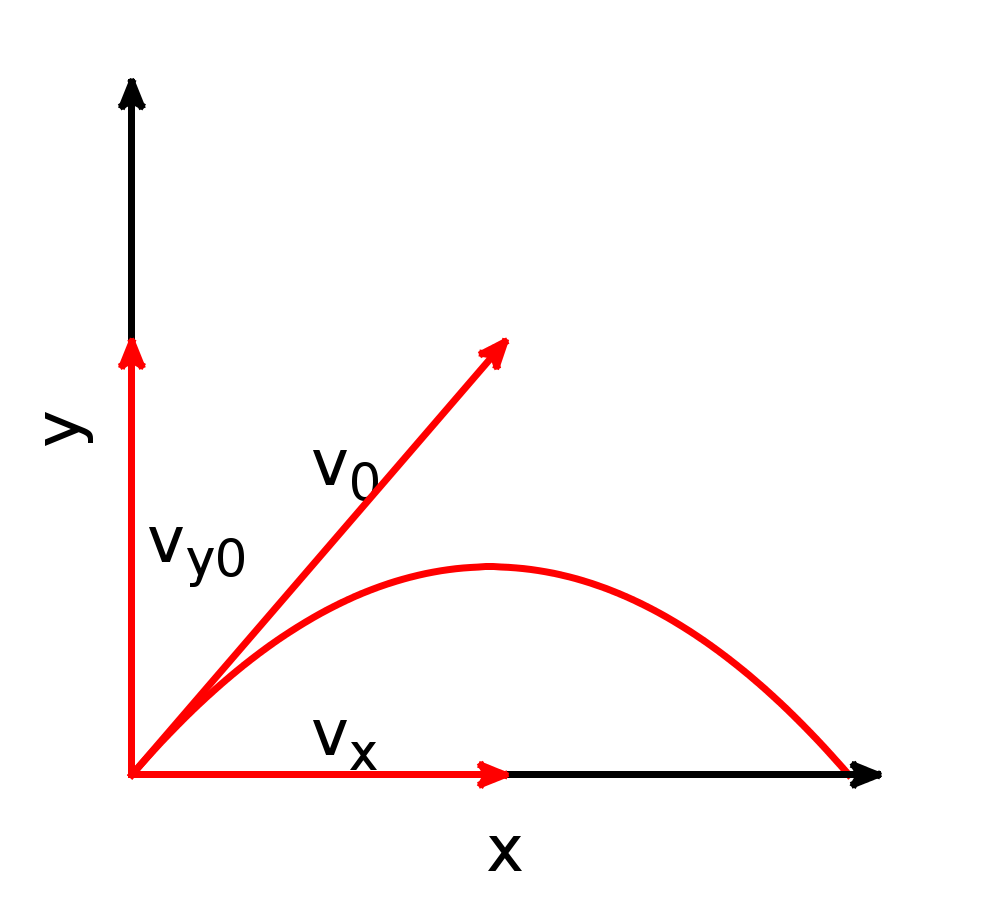
\includegraphics[width=0.6\textwidth]{schraeger_wurf.png}
	\caption{Geschwindigkeitsbeziehungen beim schrägen Wurf}
	\label{fig:abwurf}
\end{figure}

Der schiefe Wurf ist prinzipiell dieselbe Kombination aus beiden Bewegungsarten wie beim waagerechten Wurf, aber mit der Schwierigkeit, dass aus dem Abwurfwinkel $\alpha$ und der Abwurfgeschwindigkeit $v_0$ erst die Anfangsgeschwindigkeiten in die beiden Richtungen, $v_x$ in Richtung des Wurfes und $v_y0$ in die Höhe, berechnet werden müssen. Die Anfangsgeschwindigkeit in y-Richtung wird deshalb nicht einfach $v_y$ genannt, weil sie, im Gegensatz von $v_x$, im Laufe des Wurfes variiert, wie in Grafik \ref{fig:abwurf}\endnote{\glqq Abwurfgrößen beim schiefen Wurf\grqq{} von Till Blaha - Eigenes Werk. Lizenziert unter Gemeinfrei.}.


\begin{align}
\begin{split}
	\cos{\alpha} &= \frac{v_x}{v_0} \\
	v_x &= \cos{\alpha} \cdot v_0
\end{split}
\end{align}

\begin{align}
\begin{split}
	\sin{\alpha} &= \frac{v_{y0}}{v_0} \\
	v_{y0} &= \sin{\alpha} \cdot v_0
\end{split}
\end{align}

\noindent Damit können die Bewegungsgesetze eingefüllt werden:

\begin{align}
\begin{split}
	x(t) &= v_x \cdot t \\
	x(t) &= \cos{\alpha} \cdot v_0 \cdot t
\end{split}
\end{align}

\begin{align}
\begin{split}
	y(t) &= -\frac{1}{2}g \cdot t^2 + v_{y0} \cdot t + y_0 \\
	y(t) &= -\frac{1}{2}g \cdot t^2 + \sin{\alpha} \cdot v_0 \cdot t + y_0
\end{split}
\end{align}


\subsubsection{Gesamtgleichung}


Jetzt kann wieder in $y(t)$ mit der nach $t$ umgestellten Gleichung für $x(t)$ ersetzt werden und man erhält die Gesamtgleichung.

\begin{align}
\begin{split}
	x(t) &= \cos{\alpha} \cdot v_0 \cdot t \\
	t(x) &= \frac{x}{\cos{\alpha} \cdot v_0}
\end{split}
\end{align}

\noindent Einsetzen:

\begin{align}
\begin{split}
	y(t) &= -\frac{1}{2}g \cdot t^2 + \sin{\alpha} \cdot v_0 \cdot t + y_0 \\
	y(x) &= -\frac{1}{2}g \cdot \frac{x^2}{\cos{^2\alpha} \cdot v_0^2} + \sin{\alpha} \cdot v_0 \cdot \frac{x}{\cos{\alpha} \cdot v_0} + y_0 \\
	y(x) &= -\frac{1}{2}g \cdot \frac{x^2}{\cos{^2\alpha} \cdot v_0^2} + \frac{\sin{\alpha} \cdot v_0 \cdot x}{\cos{\alpha} \cdot v_0} + y_0 \\
	y(x) &= -\frac{1}{2}g \cdot \frac{x^2}{\cos{^2\alpha} \cdot v_0^2} + \tan{\alpha} \cdot x + y_0 \\
\end{split}
\end{align}

\noindent Diese Gesamtgleichung kann nun zu Berechnungen benutzt werden, z.B. muss zur Wurfweitenbestimmung die Gleichung gleich $0$ gesetzt werden. 

Die fertig gekürzte Gleichung lautet:

\begin{align}
\begin{split}
	y(x) &= \tan{\alpha} \cdot x - \frac{g \cdot x^2}{2\cos{^2\alpha} \cdot v_0^2} + y_0
\end{split}
\end{align}